\documentclass{beamer}
\usepackage[T1]{fontenc}
\usepackage{ctex, hyperref}
\usepackage{graphicx}
\usepackage{amsmath}
\usepackage{hyperref}
\usepackage{amsfonts,amssymb}
\usepackage{listings} 
\usepackage{cite}
\usepackage{tikz}
\usetikzlibrary{arrows,shapes,chains}
\tikzstyle{decision} = [diamond, draw, fill=orange!80, text width=5.0em, text centered, node distance=3.1cm, ] 
\tikzstyle{document} = [rectangle, draw, fill=blue!30, text width=4.7em, text centered, node distance=2.5cm, ] 
\tikzstyle{block1} = [rectangle, draw, fill=green!50, %here, we have chosen another block for the different color
text width=4.5em, text centered, rounded corners, node distance= 3cm, minimum height=3em] % you can create as many different shapes to make your diagram more creative and attractive, depending on the requirements

\tikzstyle{block} = [rectangle, draw, fill=yellow!50, text width=4.5em, text centered, rounded corners, node distance=2.25cm, minimum height=4em]
\tikzstyle{line} = [draw, -latex']
\tikzstyle{cloud} = [draw, ellipse, text width= 2.9em, fill=red!50, node distance=2cm, minimum height=3em]

\tikzstyle{ioi} = [trapezium, draw, trapezium right angle=120, rounded corners, fill=blue!60, node distance=2.8cm, minimum height=2.7em]
 \tikzstyle{io} = [trapezium, draw, trapezium right angle=110, rounded corners, fill=red!20, node distance=1.9cm, minimum height=2.9em]   % the draw command here is used to draw the boundary of mentioned shape.
 \tikzstyle{arrow} = [thick,->,>=stealth]
\author{褚朱钇恒}
\title{一维非线性方程的求根}
\subtitle{最终项目作业}
\institute{数学软件}
\date{2022年7月4日}
\bibliographystyle{plain}
\usepackage{Tsinghua}

% defs
\def\cmd#1{\texttt{\color{red}\footnotesize $\backslash$#1}}
\def\env#1{\texttt{\color{blue}\footnotesize #1}}
\definecolor{deepblue}{rgb}{0,0,0.5}
\definecolor{deepred}{rgb}{0.6,0,0}
\definecolor{deepgreen}{rgb}{0,0.5,0}
\definecolor{halfgray}{gray}{0.55}

\lstset{
    basicstyle=\ttfamily\small,
    keywordstyle=\bfseries\color{deepblue},
    emphstyle=\ttfamily\color{deepred},    % Custom highlighting style
    stringstyle=\color{deepgreen},
    numbers=left,
    numberstyle=\small\color{halfgray},
    rulesepcolor=\color{red!20!green!20!blue!20},
    frame=shadowbox,
}

\newtheorem*{inner}{\innerheader}
\newcommand{\innerheader}{}
\renewenvironment{theorem}
 {\renewcommand\innerheader{定理\,\stepcounter{theorem}\thetheorem}\begin{inner}}
 {\end{inner}}

\begin{document}

\kaishu
\begin{frame}
    \titlepage
\end{frame}

\begin{frame}
    \tableofcontents[sectionstyle=show,subsectionstyle=show/shaded/hide,subsubsectionstyle=show/shaded/hide]
\end{frame}
\section{定义}
\begin{frame}{求解一维非线性方程}
    求解
    \begin{equation}
        f(x)=0
        \label{eq::1}
   \end{equation}
   即确定$x^*\in[a,b]$使$f(x^*)=0$,其中$f$是定义在[a,b]上的连续非线性函数,满足$f(x^*)=0$的$x^*$成为方程(\ref{eq::1})的根,也称为$f(x)$的零点。
\end{frame}

\section{数学理论}
\begin{frame}{数学理论\cite{mathematical_analysis}}
    \begin{theorem}{介值定理}
        \label{the::intermediate}
        如果$f(x)$在区间$[a,b]$上连续且$f(a)f(b)<0$,则至少存在一点$\eta\in[a,b]$使$f(\eta)=0$

   \end{theorem}
   \begin{theorem}{泰勒公式}
        \label{the::taylor}
        把$f(x)$在$x_0$点附近展开成Taylor级数,得到
        $$f(x)=f(x_0)+(x-x_0)f^{'}(x_0)+(x-x_0)^2f^{''}(x_0)+\cdots$$
   \end{theorem}
\end{frame}

\section{问题分析与算法}
\begin{frame}{二分法和牛顿法}
    由上述两个定理,可以得出二分法和牛顿法的基本想法。\cite{nb_zhihu}
    \begin{figure}[H]
        \centering
        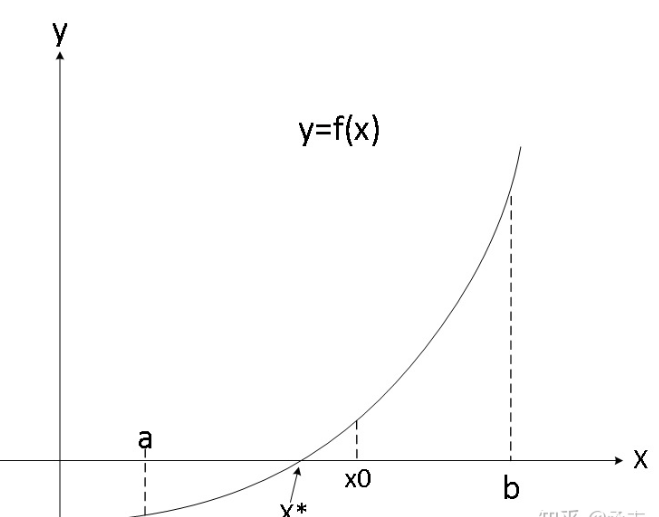
\includegraphics[scale=0.20]{./pic/1.png}
        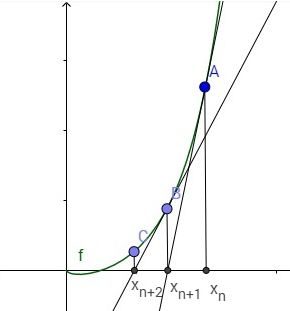
\includegraphics[scale=0.3]{./pic/2.png}
        
        \caption{二分法和牛顿法的示意图}
      \end{figure}
\end{frame}
\begin{frame}{算法流程}
    \begin{figure}[H]
        \centering
        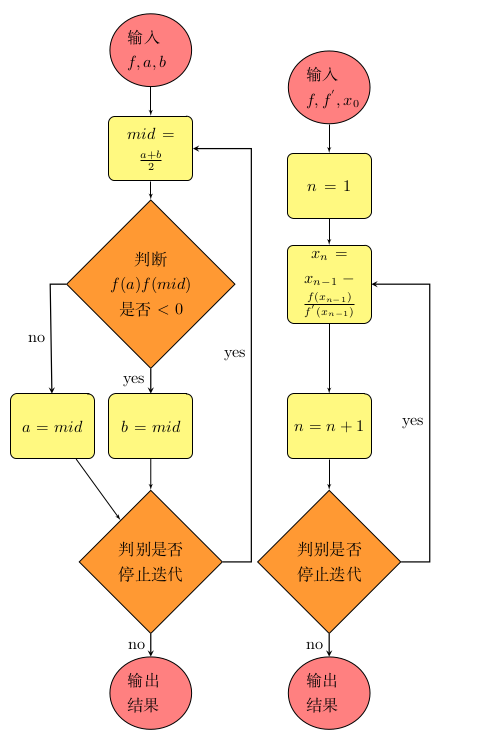
\includegraphics[scale=0.28]{./pic/3.png}
         \label{algo::1}
        \end{figure}
\end{frame}
\section{数值算例和收敛性测试}
\begin{frame}{测试}
    测试方法:随机生成100000个一维非线性方程,分别使用gsl库提供的Newton法和二分法求一个解\cite{GSL_roots}。

    \begin{figure}[H]
        \begin{center}
             \input{eg2.tex}
        \end{center}
        \label{fig::1}
        \caption{测试结果}
   \end{figure}
\end{frame}
\section{结论}
\begin{frame}{结论}
    \begin{table}[]
        \begin{tabular}{lllll}
        \cline{1-4}
        \multicolumn{1}{|l|}{}           & \multicolumn{1}{l|}{Newton法}  & \multicolumn{1}{l|}{二分法}       & \multicolumn{1}{l|}{差距}       &  \\ \cline{1-4}
        \multicolumn{1}{|l|}{求解成功率}      & \multicolumn{1}{l|}{84.76\%}  & \multicolumn{1}{l|}{72.31\%}   & \multicolumn{1}{l|}{12.45\%}  &  \\ \cline{1-4}
        \multicolumn{1}{|l|}{成功求解平均迭代次数} & \multicolumn{1}{l|}{8.190147} & \multicolumn{1}{l|}{14.506403} & \multicolumn{1}{l|}{-6.316256} &  \\ \cline{1-4}
                                         &                               &                                &                               & 
        \end{tabular}
    \end{table}

    在本次测试的场景下,牛顿法的收敛性和收敛速度都优于二分法,但从稳定性和对函数可导性的要求来看,二分法也有可取之处。
\end{frame}
\section{参考文献}
\begin{frame}{参考文献}
    \bibliography{quote}
\end{frame}

\end{document}